% Options for packages loaded elsewhere
\PassOptionsToPackage{unicode}{hyperref}
\PassOptionsToPackage{hyphens}{url}
%
\documentclass[
]{article}
\title{GLOBE Research: Leadership and Societal Perspectives}
\usepackage{etoolbox}
\makeatletter
\providecommand{\subtitle}[1]{% add subtitle to \maketitle
  \apptocmd{\@title}{\par {\large #1 \par}}{}{}
}
\makeatother
\subtitle{Stats 140XP Final Project}
\author{Ethan Allavarpu \(\cdot\) Raymond Bai \(\cdot\) Jaclyn Chiu
\(\cdot\) Ariel Chow \(\cdot\) Carlie Lin \(\cdot\) Dara
Tan \and \textbf{Explore the GLOBE}}
\date{10 December 2021}

\usepackage{amsmath,amssymb}
\usepackage{lmodern}
\usepackage{iftex}
\ifPDFTeX
  \usepackage[T1]{fontenc}
  \usepackage[utf8]{inputenc}
  \usepackage{textcomp} % provide euro and other symbols
\else % if luatex or xetex
  \usepackage{unicode-math}
  \defaultfontfeatures{Scale=MatchLowercase}
  \defaultfontfeatures[\rmfamily]{Ligatures=TeX,Scale=1}
\fi
% Use upquote if available, for straight quotes in verbatim environments
\IfFileExists{upquote.sty}{\usepackage{upquote}}{}
\IfFileExists{microtype.sty}{% use microtype if available
  \usepackage[]{microtype}
  \UseMicrotypeSet[protrusion]{basicmath} % disable protrusion for tt fonts
}{}
\makeatletter
\@ifundefined{KOMAClassName}{% if non-KOMA class
  \IfFileExists{parskip.sty}{%
    \usepackage{parskip}
  }{% else
    \setlength{\parindent}{0pt}
    \setlength{\parskip}{6pt plus 2pt minus 1pt}}
}{% if KOMA class
  \KOMAoptions{parskip=half}}
\makeatother
\usepackage{xcolor}
\IfFileExists{xurl.sty}{\usepackage{xurl}}{} % add URL line breaks if available
\IfFileExists{bookmark.sty}{\usepackage{bookmark}}{\usepackage{hyperref}}
\hypersetup{
  pdftitle={GLOBE Research: Leadership and Societal Perspectives},
  pdfauthor={Ethan Allavarpu \textbackslash cdot Raymond Bai \textbackslash cdot Jaclyn Chiu \textbackslash cdot Ariel Chow \textbackslash cdot Carlie Lin \textbackslash cdot Dara Tan; },
  hidelinks,
  pdfcreator={LaTeX via pandoc}}
\urlstyle{same} % disable monospaced font for URLs
\usepackage[margin=1in]{geometry}
\usepackage{graphicx}
\makeatletter
\def\maxwidth{\ifdim\Gin@nat@width>\linewidth\linewidth\else\Gin@nat@width\fi}
\def\maxheight{\ifdim\Gin@nat@height>\textheight\textheight\else\Gin@nat@height\fi}
\makeatother
% Scale images if necessary, so that they will not overflow the page
% margins by default, and it is still possible to overwrite the defaults
% using explicit options in \includegraphics[width, height, ...]{}
\setkeys{Gin}{width=\maxwidth,height=\maxheight,keepaspectratio}
% Set default figure placement to htbp
\makeatletter
\def\fps@figure{htbp}
\makeatother
\setlength{\emergencystretch}{3em} % prevent overfull lines
\providecommand{\tightlist}{%
  \setlength{\itemsep}{0pt}\setlength{\parskip}{0pt}}
\setcounter{secnumdepth}{-\maxdimen} % remove section numbering
\usepackage{booktabs}
\usepackage{longtable}
\usepackage{array}
\usepackage{multirow}
\usepackage{wrapfig}
\usepackage{float}
\usepackage{colortbl}
\usepackage{pdflscape}
\usepackage{tabu}
\usepackage{threeparttable}
\usepackage{threeparttablex}
\usepackage[normalem]{ulem}
\usepackage{makecell}
\usepackage{xcolor}
\usepackage{booktabs}
\usepackage{longtable}
\usepackage{array}
\usepackage{multirow}
\usepackage{wrapfig}
\usepackage{float}
\usepackage{colortbl}
\usepackage{pdflscape}
\usepackage{tabu}
\usepackage{threeparttable}
\usepackage{threeparttablex}
\usepackage[normalem]{ulem}
\usepackage{makecell}
\usepackage{xcolor}
\ifLuaTeX
  \usepackage{selnolig}  % disable illegal ligatures
\fi

\begin{document}
\maketitle

{
\setcounter{tocdepth}{1}
\tableofcontents
}
\vfill

\newpage

\hypertarget{abstract}{%
\section{Abstract}\label{abstract}}

We wanted to answer two main questions: which leadership qualities do
countries tend to view similarly and if countries align their
perceptions of societal practices and values. For determining leadership
qualities and similar countries, we used principal component analysis
(PCA) then \(k\)-means clustering to create four ``clusters'' of
countries with similar leadership beliefs. For determining the alignment
of perceptions of societal practices and values, we used linear
regression models for each pair. Then, we performed t-tests for each
dimension to check for significant slopes. We found that leadership
characteristics are generally clustered by if the trait is negative or
positive and that leadership values are clustered by region, except for
one interesting case. On the perceptions side, we shockingly discovered
that societal practices and societal values of countries do not align
and are instead opposing. In the future, we recommend looking into
causes behind the interesting disconnect between practices and values.
Some limitations to our project are the data silences due to the lack of
information from many countries.

\hypertarget{problem-statements}{%
\section{Problem Statements}\label{problem-statements}}

\begin{enumerate}
\def\labelenumi{\arabic{enumi}.}
\tightlist
\item
  Which characteristics or traits do countries tend to group together
  when determining ``good'' leadership values?

  \begin{itemize}
  \tightlist
  \item
    Which countries have similar perceptions of these leadership values?
  \end{itemize}
\item
  Do societal practices and societal values align?

  \begin{itemize}
  \tightlist
  \item
    If they do not, which practices and values deviate most
    significantly?
  \end{itemize}
\end{enumerate}

\hypertarget{description-of-dataset}{%
\section{Description of Dataset}\label{description-of-dataset}}

The data set we have chosen to analyze is the \textbf{Dana Landis
Leadership} dataset, which comes from the GLOBE Research Survey. The
data provided in the folder had survey results for (1) leadership and
(2) societal and culture data and a PDF describing the nature of the
survey, but nothing more. To glean more information, we found the two
questionnaires (alpha and beta) described in the informational PDF to
get the original questions asked in the surveys. While we do not have a
``codebook'' in a traditional sense, the original questions asked may
help guide us in understanding what each variable means and how the
survey represents respondents answers numerically. The survey is on a 1
to 7 scale. For the leadership data, 1 was a negative response, 4 a
``neutral'' score, and 7 positive. For the societal data, the
``positive'' and ``negative'' values depended on the question, but for
the relationships we analyzed, this did not impact our results.

The GLOBE (Global Leadership \& Organizational Behavior Effectiveness)
research program is an interdisciplinary study aiming to identify the
interrelationships between societal culture, societal effectiveness and
organizational leadership. Surveying from over 17,000 middle managers
from 62 cultures, the 2004 research survey provides data that measures
the leadership and societal culture practices of each country (House et
al, 2004).

A single, complete observation from the leadership survey is about a
specific culture (either a country or a subcountry) about the following
characteristics: Country; Country Name; Performance Oriented;
Autocratic; Modesty; Charismatic 3 Self sacrifice; Team 1 Collaborative
Team Orientation; Decisive; Diplomatic; Face saver; Charismatic 1
Visionary; Humane oriented; Integrity; Bureaucratic Originally Labeled
\emph{Procedural}; Administratively Competent; Self centred; Autonomous;
Status Conscious; Charismatic 2 Inspirational; Malevolent; Team 2 Team
Integrator; Internally Competitive Originally Labeled \emph{Conflict
Inducer}; Participative; Charismatic Value based Global Leadership
Dimension; Team Oriented Global Leadership Dimension; Self Protective
Global Leadership Dimension; Participative Global Leadership Dimension;
Humane Oriented Global Leadership Dimension; Autonomous Global
Leadership Dimension; Country Cluster.

A single, complete observation from the society and culture survey has a
similar structure as the leadership survey: each observation is for a
specific culture (either a country or a subcountry) about the following
characteristics: Country; Country Name; Uncertainty Avoidance Societal
Practices; Future Orientation Societal Practices; Power Distance
Societal Practices; Collectivism I Societal Practices Institutional
Collectivism ; Humane Orientation Societal Practices; Performance
Orientation Societal Practices; Collectivism II Societal Practices In
group Collectivism ; Gender Egalitarianism Societal Practices;
Assertiveness Societal Practices; Uncertainty Avoidance Societal Values;
Future Orientation Societal Values; Power Distance Societal Values;
Collectivism I Societal Values Institutional Collectivism ; Human
Orientation Societal Values; Performance Orientation Societal Values;
Collectivism II Societal Values In group Collectivism ; Gender
Egalitarianism Societal Values; Assertiveness Societal Values; Country
Cluster.

\hypertarget{visualization-and-exploratory-data-analysis}{%
\section{Visualization and Exploratory Data
Analysis}\label{visualization-and-exploratory-data-analysis}}

\hypertarget{leadership}{%
\subsection{Leadership}\label{leadership}}

\begin{center}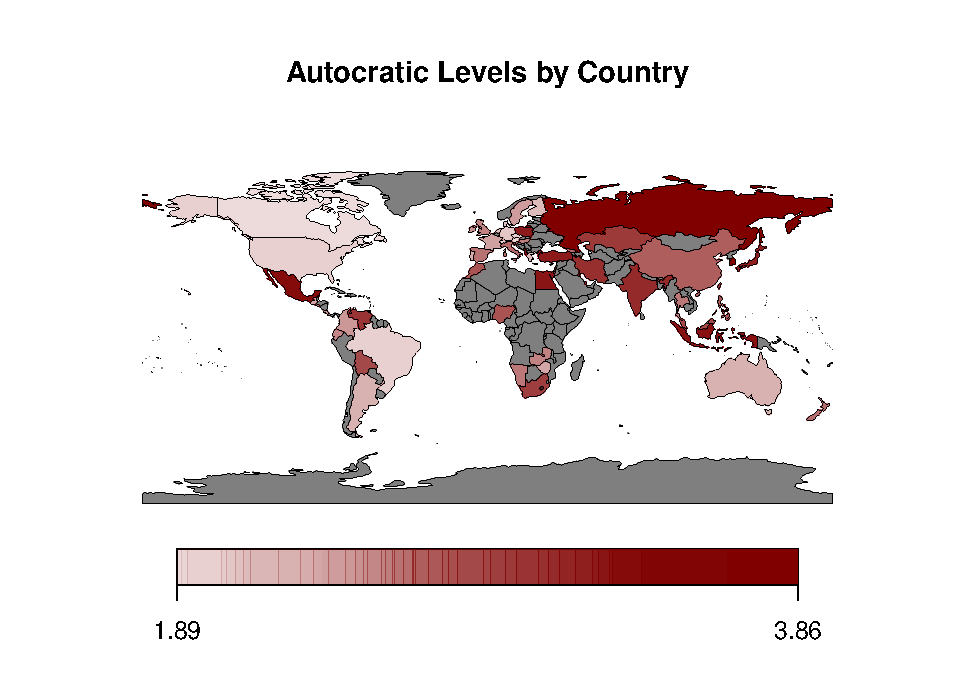
\includegraphics[width=0.95\linewidth]{report_files/figure-latex/leadership-1} \end{center}

The above map shows autocratic levels by country. The lighter colors
correspond with lower levels of autocracy while the darker colors
correspond with higher levels of autocracy. For example, we see that
Russia, a well-known autocratic country, is shaded darkly. Notably,
there do seem to be clusters of autocratic countries in the East and
clusters of less autocratic countries in the West. The East is known for
being more collectivist while the West is known for being more
individualistic. As we delve into later, beliefs and cultures do seem to
vary by region.

From boxplots we generated (not pictured), the difference by country
cluster (as defined by the dataset) seems visible, prompting us to
consider clustering countries to determine how they may be separated. We
do want to note that there are only 62 observations--this totals to
fewer than 62 countries because Germany and South Africa have two
observations each (West vs.~East and White vs.~Black, respecively). The
limited number of observations may limit us in the scope of our analysis
because we have less than a third of the total countries (demonstrated
by the vast swaths of grey on the world map for which there is no data)
and clustering would further reduce block/group sizes.

\hypertarget{societal-values-and-practices}{%
\subsection{Societal Values and
Practices}\label{societal-values-and-practices}}

\begin{center}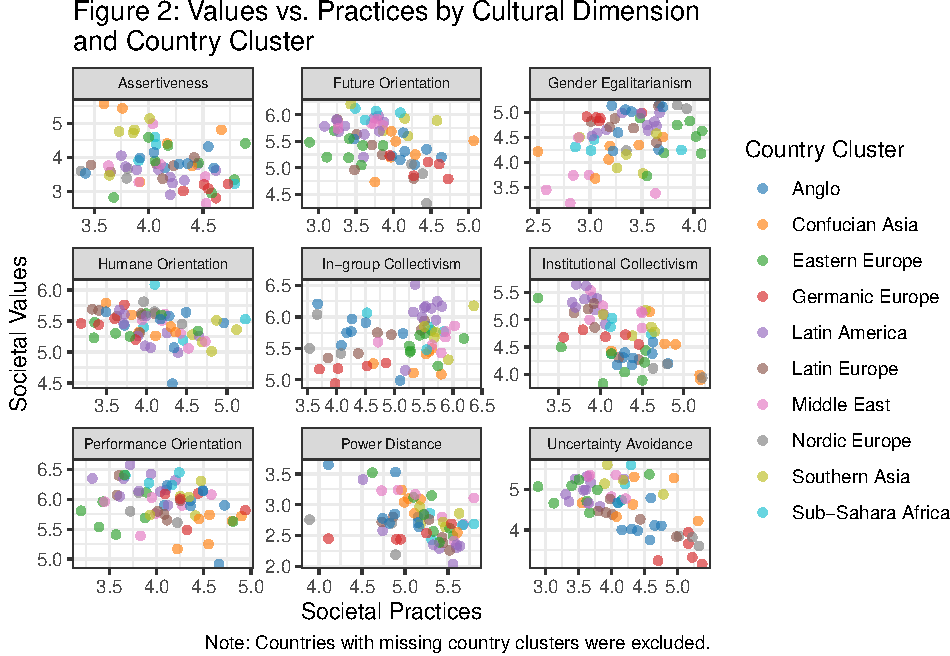
\includegraphics[width=0.85\linewidth]{report_files/figure-latex/society-1} \end{center}

The plot grid demonstrates how, contrary to what \emph{should} happen,
the societal values of a country do not correlate well with the societal
practices (what \emph{should be} does not align with what \emph{is}).
This may be a source of further exploration, as we may want to see
whether there is a significant difference between the values and
practices. When we look at the per-region divisions though (by color),
the trend (or lack thereof) seems to persist for these concepts.

\hypertarget{analysis}{%
\section{Analysis}\label{analysis}}

\hypertarget{leadership-values}{%
\subsection{Leadership Values}\label{leadership-values}}

For the leadership values problem statement, the first objective is to
collapse the data into the first four principal components through
principal component analysis (PCA). PCA finds the directions which
capture the most variability (spread) in the data--the first four
account for the maximum variation. PCA allows us to visualize trends in
the leadership values: countries tend to have similar sentiments about
variables that ``point'' in the same direction (had principal component
values that aligned).

Before performing PCA, though, we remove the second-order factor
analysis variables due to the heavy correlation with the original
predictor variables and a more difficult interpretation of these
variables. Since our goal is to understand the relationship between
certain leadership characteristics, keeping these complicated variables
might reduce our understanding and make interpretation more difficult.

After performing PCA, we perform \(k\)-means clustering on the first
four principal components to determine the ``groups'' of leadership
characteristics that have similar perceptions. \(K\)-means clustering
creates \(k\) groups that are the ``most similar'' to the other
observations in their groups, minimizing the between-group variability:

\definecolor{clust3}{HTML}{408000}
\definecolor{clust2}{HTML}{800080}
\definecolor{clust1}{HTML}{008080}

\begin{enumerate}
\def\labelenumi{\arabic{enumi}.}
\tightlist
\item
  \textcolor{clust1}{Internally competitive, malevolent, status conscious, self-centred, bureaucratic, face saver, autocratic}
\item
  \textcolor{clust2}{Humane-oriented, modesty}
\item
  \textcolor{clust3}{Participative, team integrator, inspirational, autonomous, administratively competent, integrity, visionary, diplomatic, decisive, collaborative team orientation, self-sacrifice, performance-oriented}
\end{enumerate}

\begin{center}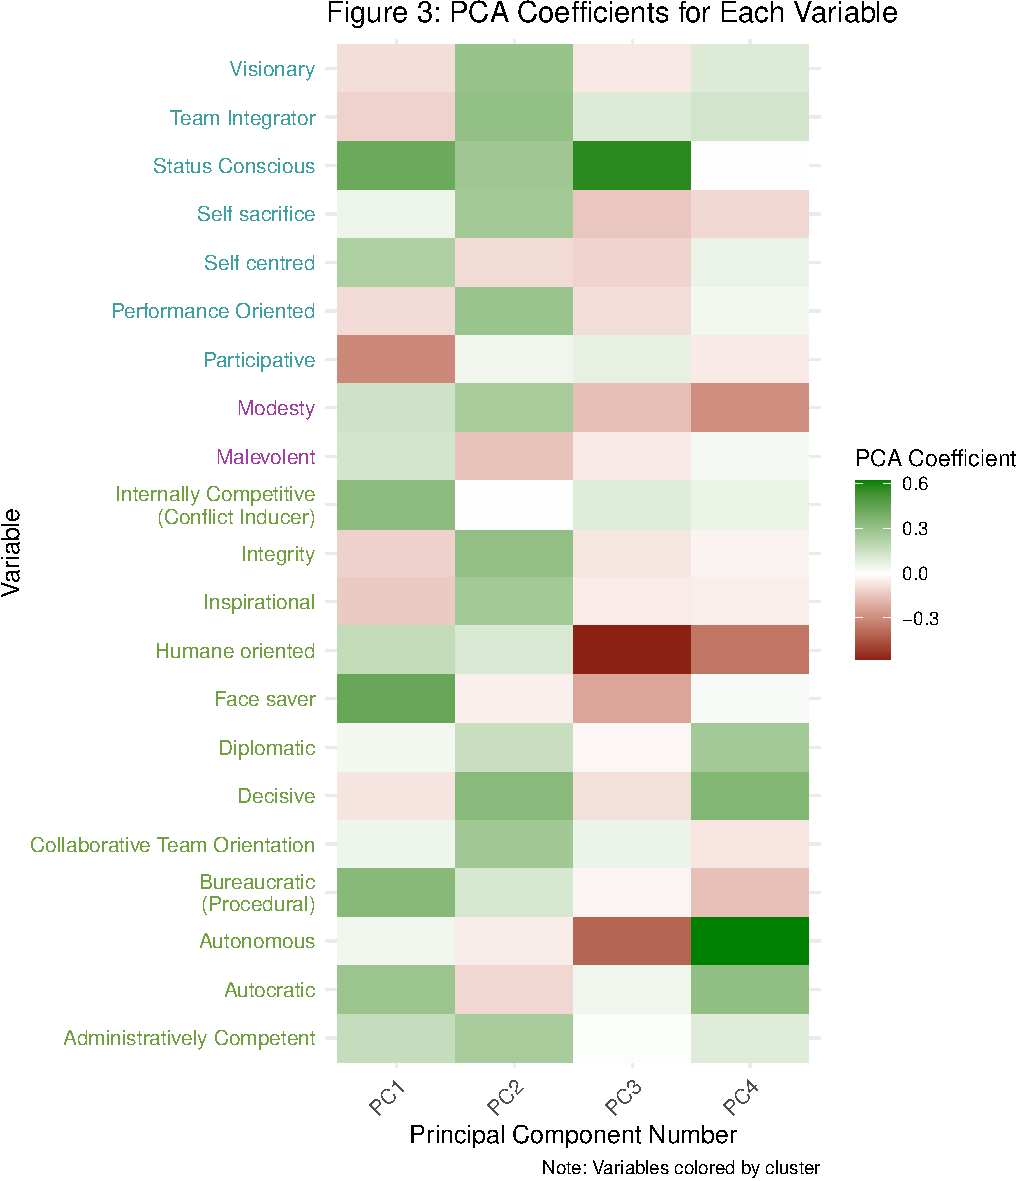
\includegraphics[width=0.85\linewidth]{report_files/figure-latex/pca_heatmap-1} \end{center}

The green cluster seems to describe positive characteristics (e.g.,
participative, inspirational), while the blue cluster appears to
describe negative characteristics (e.g., malevolent, self-centered).
From this, we note that these ``positive'' and ``negative''
characteristics tend to occur together. The third ``cluster'' (i.e.,
humane oriented and modesty) did not closely fit with the other groups,
leading us to believe that they may be considered separately from the
other characteristics.

After considering the leadership characteristics, we cluster countries
based on similar perceptions. We do this by using the variables of the
countries transformed into the first four principal components, then
running \(k\)-means clustering on those components. The clustering
results segregate the countries into the following segments:

\begin{center}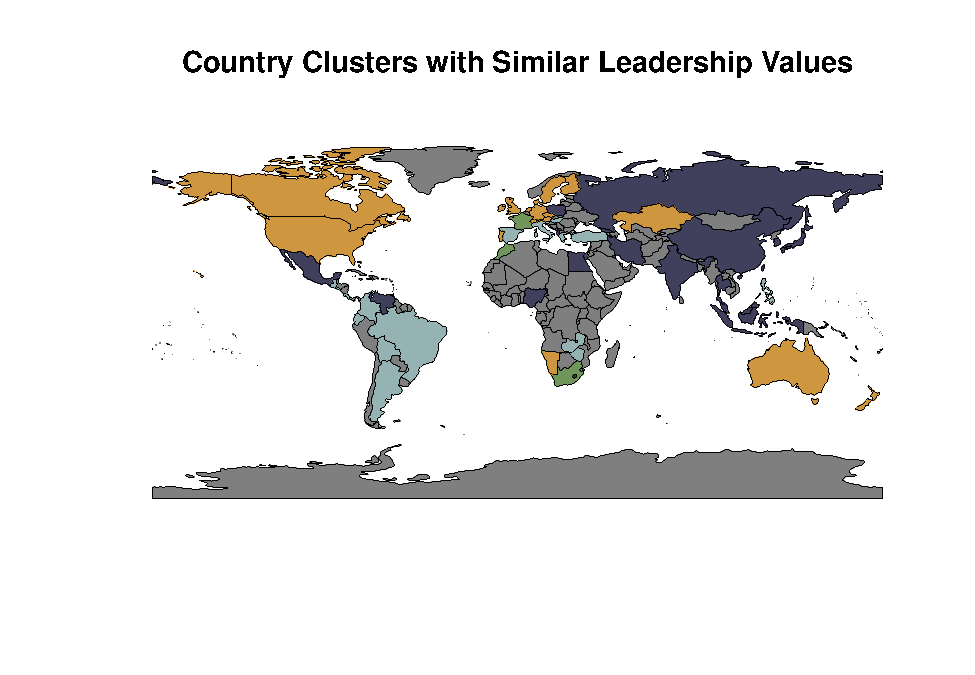
\includegraphics[width=0.95\linewidth]{report_files/figure-latex/kmeans-1} \end{center}

\begin{table}[h]

\caption{\label{tab:country_table}Regions with Similar Leadership Perceptions}
\centering
\begin{tabular}[t]{>{}l>{}l>{}l>{}l}
\toprule
Cluster 1 & Cluster 2 & Cluster 3 & Cluster 4\\
\midrule
\textcolor[HTML]{739999}{\cellcolor{gray!6}{Argentina}} & \textcolor[HTML]{000026}{\cellcolor{gray!6}{Albania}} & \textcolor[HTML]{407326}{\cellcolor{gray!6}{France}} & \textcolor[HTML]{BF7300}{\cellcolor{gray!6}{Australia}}\\
\textcolor[HTML]{739999}{Bolivia} & \textcolor[HTML]{000026}{China} & \textcolor[HTML]{407326}{Morocco} & \textcolor[HTML]{BF7300}{Austria}\\
\textcolor[HTML]{739999}{\cellcolor{gray!6}{Brazil}} & \textcolor[HTML]{000026}{\cellcolor{gray!6}{Egypt}} & \textcolor[HTML]{407326}{\cellcolor{gray!6}{Qatar}} & \textcolor[HTML]{BF7300}{\cellcolor{gray!6}{Canada (English-speaking)}}\\
\textcolor[HTML]{739999}{Colombia} & \textcolor[HTML]{000026}{Georgia} & \textcolor[HTML]{407326}{South Africa (Black Sample)} & \textcolor[HTML]{BF7300}{Czech Republic}\\
\textcolor[HTML]{739999}{\cellcolor{gray!6}{Costa Rica}} & \textcolor[HTML]{000026}{\cellcolor{gray!6}{Hong Kong}} & \textcolor[HTML]{407326}{\cellcolor{gray!6}{}} & \textcolor[HTML]{BF7300}{\cellcolor{gray!6}{Denmark}}\\
\addlinespace
\textcolor[HTML]{739999}{Ecuador} & \textcolor[HTML]{000026}{India} & \textcolor[HTML]{407326}{} & \textcolor[HTML]{BF7300}{England}\\
\textcolor[HTML]{739999}{\cellcolor{gray!6}{El Salvador}} & \textcolor[HTML]{000026}{\cellcolor{gray!6}{Indonesia}} & \textcolor[HTML]{407326}{\cellcolor{gray!6}{}} & \textcolor[HTML]{BF7300}{\cellcolor{gray!6}{Finland}}\\
\textcolor[HTML]{739999}{Greece} & \textcolor[HTML]{000026}{Iran} & \textcolor[HTML]{407326}{} & \textcolor[HTML]{BF7300}{French Switzerland}\\
\textcolor[HTML]{739999}{\cellcolor{gray!6}{Guatemala}} & \textcolor[HTML]{000026}{\cellcolor{gray!6}{Japan}} & \textcolor[HTML]{407326}{\cellcolor{gray!6}{}} & \textcolor[HTML]{BF7300}{\cellcolor{gray!6}{Germany (EAST)}}\\
\textcolor[HTML]{739999}{Hungary} & \textcolor[HTML]{000026}{Kuwait} & \textcolor[HTML]{407326}{} & \textcolor[HTML]{BF7300}{Germany (WEST)}\\
\addlinespace
\textcolor[HTML]{739999}{\cellcolor{gray!6}{Israel}} & \textcolor[HTML]{000026}{\cellcolor{gray!6}{Malaysia}} & \textcolor[HTML]{407326}{\cellcolor{gray!6}{}} & \textcolor[HTML]{BF7300}{\cellcolor{gray!6}{Ireland}}\\
\textcolor[HTML]{739999}{Italy} & \textcolor[HTML]{000026}{Mexico} & \textcolor[HTML]{407326}{} & \textcolor[HTML]{BF7300}{Kazakhstan}\\
\textcolor[HTML]{739999}{\cellcolor{gray!6}{Philippines}} & \textcolor[HTML]{000026}{\cellcolor{gray!6}{Nigeria}} & \textcolor[HTML]{407326}{\cellcolor{gray!6}{}} & \textcolor[HTML]{BF7300}{\cellcolor{gray!6}{Namibia}}\\
\textcolor[HTML]{739999}{Slovenia} & \textcolor[HTML]{000026}{Poland} & \textcolor[HTML]{407326}{} & \textcolor[HTML]{BF7300}{Netherlands}\\
\textcolor[HTML]{739999}{\cellcolor{gray!6}{Spain}} & \textcolor[HTML]{000026}{\cellcolor{gray!6}{Russia}} & \textcolor[HTML]{407326}{\cellcolor{gray!6}{}} & \textcolor[HTML]{BF7300}{\cellcolor{gray!6}{New Zealand}}\\
\addlinespace
\textcolor[HTML]{739999}{Turkey} & \textcolor[HTML]{000026}{South Korea} & \textcolor[HTML]{407326}{} & \textcolor[HTML]{BF7300}{Portugal}\\
\textcolor[HTML]{739999}{\cellcolor{gray!6}{Zambia}} & \textcolor[HTML]{000026}{\cellcolor{gray!6}{Taiwan}} & \textcolor[HTML]{407326}{\cellcolor{gray!6}{}} & \textcolor[HTML]{BF7300}{\cellcolor{gray!6}{Singapore}}\\
\textcolor[HTML]{739999}{Zimbabwe} & \textcolor[HTML]{000026}{Thailand} & \textcolor[HTML]{407326}{} & \textcolor[HTML]{BF7300}{South Africa (White Sample)}\\
\textcolor[HTML]{739999}{\cellcolor{gray!6}{}} & \textcolor[HTML]{000026}{\cellcolor{gray!6}{Venezuela}} & \textcolor[HTML]{407326}{\cellcolor{gray!6}{}} & \textcolor[HTML]{BF7300}{\cellcolor{gray!6}{Sweden}}\\
\textcolor[HTML]{739999}{} & \textcolor[HTML]{000026}{} & \textcolor[HTML]{407326}{} & \textcolor[HTML]{BF7300}{Switzerland}\\
\addlinespace
\textcolor[HTML]{739999}{\cellcolor{gray!6}{}} & \textcolor[HTML]{000026}{\cellcolor{gray!6}{}} & \textcolor[HTML]{407326}{\cellcolor{gray!6}{}} & \textcolor[HTML]{BF7300}{\cellcolor{gray!6}{USA}}\\
\bottomrule
\end{tabular}
\end{table}

\emph{Note: East and West Germany belong to the same cluster and are
colored as such. South Africa is colored by the cluster the Black sample
belongs in, rather than the White sample. Countries that are not
included in the data are colored gray.}

From the above grouping, we see that regionality (generally) determines
a country's respective cluster and leadership perspectives. Cluster 1
(light blue) tends to describe Latin American and the Mediterranean,
Cluster 2 (dark blue) generally includes Asia, and Cluster 4 (gold)
describes the Anglo regions and northern Europe. The one cluster that
appears to be ``out there'' is Cluster 3 (green), which does not have a
particular region associated with it. To visualize the differences
between these clusters, we create a heatmap of the median variable
values for each cluster:

\begin{center}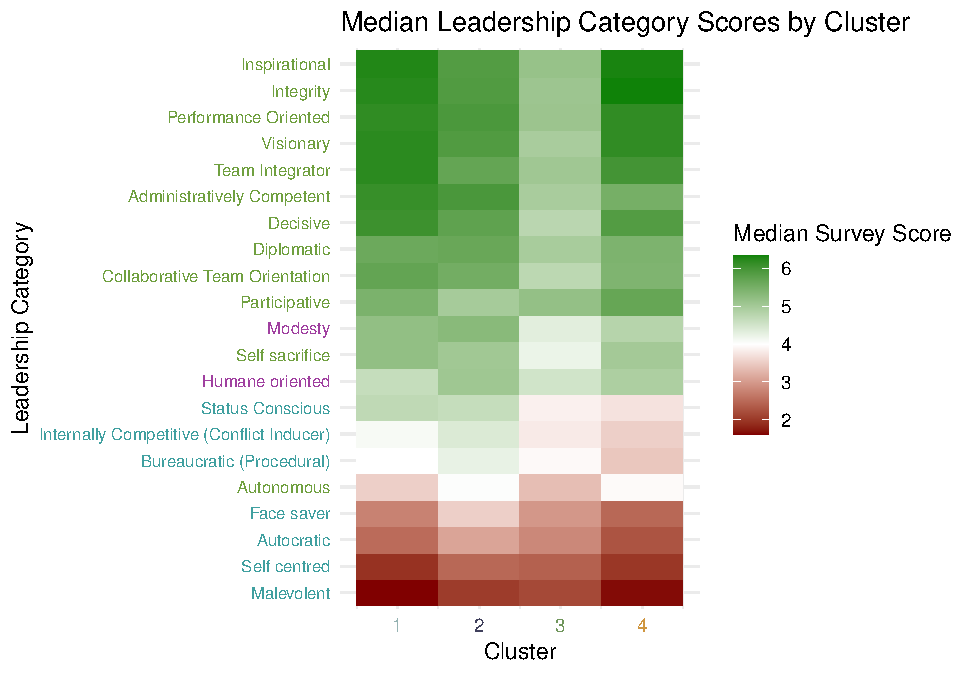
\includegraphics[width=0.85\linewidth]{report_files/figure-latex/cluster_values-1} \end{center}

From here, we see that, despite the clustering, the countries tend to
agree on beneficial and detrimental leadership qualities; the main
difference is in the intensity: clusters 1 and 4 seem to have the
strongest responses (most positive and most negative), while cluster 3
does not seem to feel terribly strongly about positive leadership
characteristics. The few qualities of intrigue, though, are the ones for
which some clusters viewed positively (green) while others viewed
negatively (red):

\begin{itemize}
\tightlist
\item
  Status Conscious
\item
  Internally Competitive (Conflict Inducer)
\item
  Bureaucratic (Procedural)
\item
  Autonomous
\end{itemize}

\hypertarget{societal-practices-and-values}{%
\subsection{Societal Practices and
Values}\label{societal-practices-and-values}}

From the scatterplots above, we note that societal practices and
societal values do not always align. For instance, in the case of the
Humane Orientation cultural dimension, there does not appear to be any
correlation between practices and values at all, with societal practices
in this dimension varying from less than 3.5 to more than 5.0 on the
survey's seven-point scale even though societal values were rated
relatively similarly across all of the surveyed countries. In some other
cases, such as for the Uncertainty Avoidance cultural dimension, there
appears to be a negative correlation between practices and values, as
indicated by the general trend of scores for practices in this dimension
decreasing even as scores for values increase. This negative correlation
might suggest that, rather than aligning, societal practices and
societal values are in fact in conflict.

To quantify the observations we made from our scatterplots above, we fit
simple linear regression models for each of the nine cultural
dimensions, using the societal values rating as the predictor and the
societal practices rating as the response. In other words, we fit the
model:

\[
y = \beta_0 + \beta_1 x
\]

Where \(x\) is the societal values rating and \(y\) is the societal
practices rating for each of the nine cultural dimensions. Additionally,
we performed \(t\)-tests for each dimension, to test the hypotheses
\(H_0: \beta_1 = 0\) and \(H_1: \beta_1 \ne 0\). For this, we employed
the \emph{Bonferroni correction} to change the significance threshold
from \(\alpha = 0.05\) to \(\alpha = \frac{0.05}{9} \approx 0.0056\)
since maintaining a significance level of \(\alpha = 0.05\) would
increase the experiment-wise error rate:
\(P(\text{Any False Positive}) = 1 - P(\text{No False Positives}) = 1 - 0.95^{9} \approx 0.3698\).
The table below shows the values of \(\beta_1\) that we obtained and the
corresponding p-values. Cultural dimensions for which the p-value is
lower than the corrected \(\alpha \approx 0.0056\) are indicated with
green shading.

\begin{table}[!h]

\caption{\label{tab:SPV SLR Table}Results of Simple Linear Regression by Cultural Dimension}
\centering
\begin{tabular}[t]{lrr}
\toprule
Cultural Dimension & Coefficient Value & p-value\\
\midrule
\cellcolor[HTML]{E5F5E0}{Uncertainty Avoidance} & \cellcolor[HTML]{E5F5E0}{-0.6199} & \cellcolor[HTML]{E5F5E0}{0.0000}\\
\cellcolor[HTML]{E5F5E0}{Institutional Collectivism} & \cellcolor[HTML]{E5F5E0}{-0.5251} & \cellcolor[HTML]{E5F5E0}{0.0000}\\
\cellcolor[HTML]{E5F5E0}{Power Distance} & \cellcolor[HTML]{E5F5E0}{-0.4991} & \cellcolor[HTML]{E5F5E0}{0.0006}\\
\cellcolor[HTML]{E5F5E0}{Future Orientation} & \cellcolor[HTML]{E5F5E0}{-0.4725} & \cellcolor[HTML]{E5F5E0}{0.0009}\\
Humane Orientation & -0.5944 & 0.0116\\
\addlinespace
\cellcolor[HTML]{F0F0F0}{Gender Egalitarianism} & \cellcolor[HTML]{F0F0F0}{0.2437} & \cellcolor[HTML]{F0F0F0}{0.0124}\\
Performance Orientation & -0.3459 & 0.0268\\
\cellcolor[HTML]{F0F0F0}{Assertiveness} & \cellcolor[HTML]{F0F0F0}{-0.1507} & \cellcolor[HTML]{F0F0F0}{0.0414}\\
In-group Collectivism & 0.4393 & 0.0991\\
\bottomrule
\end{tabular}
\end{table}

As shown above, most of the \(\beta_1\) values obtained were negative,
including all four values that were significant at the
\(\alpha = 0.56\)\% significant level as calculated using the Bonferroni
correction. This means that, as the rating for the societal values of a
cultural dimension increase, the rating for the societal practices of
that cultural dimension actually decrease. In other words, rather than
being aligned, societal practices in fact run counter to societal
values.

\hypertarget{conclusions}{%
\section{Conclusions}\label{conclusions}}

Leadership characteristics are largely clustered based on whether each
trait is negative or positive. For example, the traits malevolent and
self centered have similar ratings while the traits integrity and
inspiration also have similar ratings. Additionally, leadership values
tend to be clustered based on their geographic region. This suggests
countries within smaller distances of one another have similar more
related leadership perspectives.

Our findings indicate that the societal practices and societal values of
countries do not align and are instead opposing. Thus, we conclude that
a country's societal value does not entail the same practices being
practiced among its constituents. This analysis can be useful for
government officials trying to develop policies that promote cultural
values. If a country places a high value on uncertainty avoidance (the
desire to rely on social norms and procedures to avoid unpredictable
events), then the same country may undergo unexpected and unconventional
events in the future.

\hypertarget{suggestions-for-further-research}{%
\section{Suggestions for Further
Research}\label{suggestions-for-further-research}}

Regarding the leadership investigation, some further research we may
consider is investigating \emph{why} Cluster 3 differs so greatly from
the other three clusters. In Cluster 3 we have France, Qatar, Morocco,
and South Africa (Black Sample). Understanding why these countries are
so different may help us see if there is an underlying link. Similarly,
we may want to consider the differences between South Africa's Black and
White samples and Germany's East and West samples. Since the survey was
conducted in 2006, Apartheid and the Berlin Wall, respectively, may play
a role in any potential differences. Ultimately, the above two
suggestions relate to us considering the country's framework: looking at
other indices (such as a freedom index, government approval ratings, or
a happiness index) could shift us from an unsupervised learning
situation (just understanding relationships between variables) to a
model-building mindset in which we might determine which characteristics
seem to have associations with more freedom/approval/happiness.

For both leadership and the societal analyses, further research may be
conducting more surveys to look at the potential changes in ideology and
perspectives over time to understanding the changing dynamics at both
the national and global level. Researchers should also look into the
potential causes behind the inverse relationship between social values
and practices.

\hypertarget{limitations}{%
\section{Limitations}\label{limitations}}

In the dataset, there are only 62 countries observed, limiting the
significance of the analysis and the confidence we have in clustering
countries by geographical similarities. In addition, there is no
explanation as to why only certain countries were surveyed. We also
recognize that at the time of data collection, the Apartheid and the
Berlin Wall potentially played significant factors in the differing
valuations of social and leadership values for citizens in South Africa
and Germany, respectively. It is notable that East and West Germany are
split up and South Africa is also split up by race.

\end{document}
